% Copyright 2026 Sreeram Anil
% SPDX-License-Identifier: CC-BY-4.0
\chapter{Auxiliary particle filter (PF-Auxiliary)}
\label{ch:pfauxiliary}

\section*{At a glance}
\begin{tabular}{@{}l>{\raggedright\arraybackslash}p{0.76\textwidth}@{}}
Family & Sequential Monte Carlo (particle / ensemble / Gaussian sum) \\
Header & \texttt{include/estkit/particle/pf\_auxiliary.hpp} \\
Registered name & \texttt{PF-Auxiliary} ($N=500$ particles) \\
State dimension & $n_x = 4$ (cell model) — generic in $n_x, n_u, n_y$ \\
Cost per step & \SI{104.4}{\micro\second}/step ($219\times$ EKF; $3N$ model evaluations) \\
Memory & \SI{54.6}{\kilo\byte} (particles, predicted means, four $N$-vectors) \\
Primary references & \cite{pitt1999auxiliary,arulampalam2002,gordon1993,cappe2007overview} \\
\end{tabular}

\section{Motivation and aerospace/BMS relevance}
The bootstrap filter propagates first and looks at the measurement afterwards.  When the likelihood
is much sharper than the one-step predictive --- the defining feature of the battery problem, where
\SI{2}{\milli\volt} of voltage noise resolves SOC to \num{0.003} while the one-step SOC uncertainty
is $10^{-5}$ --- almost every particle is propagated into a region that the new measurement then
rejects.  The computation spent on those particles is wasted twice over: once in evaluating $f$ for
a sample that will get zero weight, and once in the variance that the resulting near-degenerate
weight vector injects into the estimate.

Pitt and Shephard \cite{pitt1999auxiliary} invert the order of operations.  They resample
\emph{before} propagating, using a cheap preview of how well each parent is likely to explain the
new measurement, so that the children are born where the likelihood already is.  The mechanism is
an auxiliary variable --- the parent index itself --- promoted to a component of the sampling
space, hence "auxiliary particle filter".  In the limit of small process noise the preview becomes
exact and the filter is \emph{fully adapted}: the second-stage weights are constant and the
estimator attains the variance of an i.i.d.\ sample from the posterior.

That limit is the operating point of a battery filter, which makes the APF a natural candidate
here, and the benchmark bears it out: \estname{PF-Auxiliary} has the best results of the four
full-state particle filters on every scenario in which the model is biased, and the lowest
steady-state SOC error of the whole family on the electrochemical plant.  The same reasoning applies to any aerospace estimator whose
measurement is far more informative per step than its dynamics are uncertain --- carrier-phase GNSS
attitude, star-tracker-aided gyro propagation, or Coulomb counting aided by a precise voltage
sensor.

\section{Problem statement and assumptions}
The model is \eqref{eq:pfb-dyn}--\eqref{eq:pfb-meas}.  In addition to the bootstrap requirements
(A1)--(A2) of Chapter~\ref{ch:pfbootstrap}, the APF needs
\begin{quote}
(A4) a cheap, deterministic \emph{characterisation} $\bm{\mu}_k^i$ of the predictive density
$p(\vx_k\mid\vx_{k-1}^i)$ --- its mean, its mode, or a single draw --- at which the likelihood can
be evaluated before the propagation noise is drawn.
\end{quote}
The implementation uses the mean, $\bm{\mu}_k^i = f(\vx_{k-1}^i, \vu_{k-1})$, which is the usual
choice \cite[eq.~(67)]{arulampalam2002} and costs one evaluation of $f$ that the time update needs
anyway.  Nothing in the derivation requires $\bm{\mu}^i$ to be a good characterisation: a poor one
degrades efficiency, not correctness, because the second-stage weights correct for whatever was
used.

\section{Derivation}

\subsection{The auxiliary variable}
Target the \emph{joint} density of the state and its parent index,
\begin{equation}
  p(\vx_k, i \mid \vy_{1:k}) \;\propto\; p(\vy_k \mid \vx_k)\, p(\vx_k \mid \vx_{k-1}^i)\, w_{k-1}^i ,
  \label{eq:apf-joint}
\end{equation}
whose marginal in $\vx_k$ is the filtering density we want.  Sampling \eqref{eq:apf-joint}
directly is no easier than before, so introduce the importance density
\begin{equation}
  q(\vx_k, i \mid \vy_{1:k}) \;\propto\; \underbrace{p(\vy_k\mid\bm{\mu}_k^i)\, w_{k-1}^i}_{\text{choose the parent}}
                                          \;\underbrace{p(\vx_k\mid\vx_{k-1}^i)}_{\text{propagate}} ,
  \label{eq:apf-q}
\end{equation}
i.e.\ pick the parent in proportion to how well its predicted mean explains $\vy_k$, then propagate
it with the ordinary transition density.  Both factors are easy: the first is a discrete
distribution on $N$ points, the second is the bootstrap proposal.

\subsection{The two-stage weights}
The importance weight of the joint sample $(\vx_k^j, i_j)$ is the ratio of \eqref{eq:apf-joint} to
\eqref{eq:apf-q}, in which the transition density and the prior weight cancel:
\begin{equation}
  \boxed{\;
  \tilde w_k^j \;=\;
  \frac{p(\vy_k\mid\vx_k^j)\, p(\vx_k^j\mid\vx_{k-1}^{i_j})\, w_{k-1}^{i_j}}
       {p(\vy_k\mid\bm{\mu}_k^{i_j})\, w_{k-1}^{i_j}\, p(\vx_k^j\mid\vx_{k-1}^{i_j})}
  \;=\; \frac{p(\vy_k\mid\vx_k^j)}{p(\vy_k\mid\bm{\mu}_k^{i_j})} \; }
  \label{eq:apf-w2}
\end{equation}
\cite[eq.~(69)]{arulampalam2002}.  The algorithm is therefore
\begin{align}
  \text{first stage:}\quad & \lambda^i \;\propto\; w_{k-1}^i\, p(\vy_k\mid\bm{\mu}_k^i),
    \qquad \textstyle\sum_i \lambda^i = 1, \label{eq:apf-first}\\
  & \{i_j\}_{j=1}^N \sim \text{systematic resampling from } \{\lambda^i\}, \nonumber\\
  \text{propagation:}\quad & \vx_k^j \sim p(\vx_k \mid \vx_{k-1}^{i_j}) = \N{\bm{\mu}_k^{i_j}}{\mQ}, \label{eq:apf-prop}\\
  \text{second stage:}\quad & w_k^j \;\propto\; p(\vy_k\mid\vx_k^j) \big/ p(\vy_k\mid\bm{\mu}_k^{i_j}).
  \label{eq:apf-second}
\end{align}

\subsection{Why this reduces the weight variance}
Two readings of \eqref{eq:apf-w2} explain the gain.

\emph{Look-ahead resampling.}  In the bootstrap filter, resampling at step $k-1$ uses information
up to $k-1$ only, so particles are duplicated on the strength of stale evidence and then killed by
$\vy_k$.  In the APF, duplication is decided with $\vy_k$ already in hand: parents whose predicted
observation is far from $\vy_k$ are eliminated \emph{before} anyone pays for their propagation.

\emph{Near-perfect adaptation.}  Suppose the process noise is small enough that
$p(\vx_k\mid\vx_{k-1}^i)$ concentrates near $\bm{\mu}_k^i$ on the scale over which
$p(\vy_k\mid\cdot)$ varies.  Then $p(\vy_k\mid\vx_k^j)\approx p(\vy_k\mid\bm{\mu}_k^{i_j})$ and
\eqref{eq:apf-w2} gives $\tilde w_k^j \approx 1$ for every $j$: the cloud is equally weighted,
$N_{\mathrm{eff}} \approx N$, and the estimator has the variance of $N$ independent draws from the
posterior.  The filter is then said to be \emph{fully adapted} \cite[\S3.2]{pitt1999auxiliary}.
Conversely, when the process noise is large the ratio in \eqref{eq:apf-w2} varies wildly and the
APF can be \emph{worse} than the bootstrap filter --- Pitt and Shephard note this explicitly, and
it is the reason the APF is not a universal replacement.

For the cell model the first regime holds by a wide margin: the one-step SOC standard deviation is
$10^{-5}$ while the likelihood width in SOC units is \num{0.003}, a ratio of \num{300}.

\subsection{Interaction with roughening}
Section~\ref{sec:pfb-battery} showed that a battery particle filter must inject artificial process
noise or its SOC cloud freezes.  In the APF that noise is folded into the propagation
\eqref{eq:apf-prop}, i.e.\ the transition covariance actually used is
\begin{equation}
  \mQ_{\mathrm{eff}} = \mQ + \diag(\sigma_1^2,\dots,\sigma_{n_x}^2),
  \qquad
  \sigma_k = \operatorname{clip}\big(K E_k N^{-1/n_x};\ \varphi_{\min}\sqrt{(\mP_0)_{kk}},\ \varphi_{\max}\sqrt{(\mP_0)_{kk}}\big),
  \label{eq:apf-qeff}
\end{equation}
exactly as in \eqref{eq:pfb-roughen-clip}.  Because the same $\mQ_{\mathrm{eff}}$ appears in the
proposal and in the (implicit) transition density, the cancellation in \eqref{eq:apf-w2} is still
exact --- the jitter is a statement about the model, not a perturbation of the sampler.  Note that
the APF resamples at \emph{every} step by construction, so the jitter acts at every step rather
than only when $N_{\mathrm{eff}}$ collapses; the default floor is therefore lowered to
$\varphi_{\min} = 0.002$ and the spread-proportional term switched off ($K=0$), which measurement
showed to be the best compromise (on the development run with $K = 0.2$ the nominal steady-state error rose by a
factor of three).

\section{Algorithm}
\begin{algorithm}[H]
\caption{PF-Auxiliary --- one sampling period}
\begin{algorithmic}[1]
\Require particles $\{\vx_{k-1}^i\}$, weights $\{w_{k-1}^i\}$, $\vu_{k-1},\vu_k,\vy_k$
\State \textbf{Time update (\code{predict}, no noise yet).}
\State $\bm\sigma \gets$ roughening scale \eqref{eq:apf-qeff}; \; $\mL_Q \gets \operatorname{chol}(\mQ(\xhat,\vu_{k-1}) + \diag(\bm\sigma^2))$
\For{$i=1$ \textbf{to} $N$} \State $\bm{\mu}^i \gets f(\vx_{k-1}^i, \vu_{k-1})$ \EndFor
\State \textbf{Prior predictive.} $\yhat_k \gets \sum_i w^i_{k-1} h(\bm{\mu}^i, \vu_k)$
\State \textbf{First stage (\code{update}).}
\For{$i=1$ \textbf{to} $N$} \State $g^i \gets \log \N{\vy_k - h(\bm{\mu}^i,\vu_k)}{\mR}$; \; $\log\lambda^i \gets \log w_{k-1}^i + g^i$ \EndFor
\State normalise $\{\lambda^i\}$; \; parents $\{i_j\}$ by systematic resampling \eqref{eq:pfb-systematic}
\State \textbf{Propagation and second stage.}
\For{$j=1$ \textbf{to} $N$}
  \State $\vx_k^j \gets \operatorname{constrain}\big(\bm{\mu}^{i_j} + \mL_Q\,\bm\xi^j\big)$, \; $\bm\xi^j\sim\N{\bm 0}{\mI}$
  \State $\log \tilde w^j \gets \log\N{\vy_k - h(\vx_k^j,\vu_k)}{\mR} - g^{i_j}$
\EndFor
\State normalise $\{\tilde w^j\} \to \{w_k^j\}$; \; $N_{\mathrm{eff}} \gets 1/\sum_j (w^j_k)^2$
\State $\xhat_k \gets \sum_j w_k^j \vx_k^j$; \; $\mP_k \gets \sum_j w_k^j (\vx_k^j - \xhat_k)(\vx_k^j-\xhat_k)^\T$
\Ensure $\xhat_k$, $\mP_k$
\end{algorithmic}
\end{algorithm}

\noindent Note that no second resampling is performed: the auxiliary stage \emph{is} the
resampling, and the second-stage weights are carried into the estimate.  Diversity is maintained by
the fact that children of the same parent receive independent draws of $\mQ_{\mathrm{eff}}$.

\subsection*{Mapping onto the \code{predict}/\code{update} interface}
The APF needs $\vy_k$ before it propagates, which the \code{CellEstimator} timing
convention --- \code{predict}$(\vu_{k-1})$, then \code{predict\_measurement}$(\vu_k)$, then
\code{update}$(\vy_k,\vu_k)$ --- does not offer directly.  The header therefore splits the time update:
\code{predict()} computes the deterministic predicted means $\bm{\mu}^i$ and the factorisation of
$\mQ_{\mathrm{eff}}$ (which need no measurement), \code{predict\_measurement()} returns
$\sum_i w^i h(\bm{\mu}^i,\vu_k)$, and \code{update()} performs stages one and two.  This is the
licensed pattern of \code{docs/ESTIMATOR\_API.md} \S3 for filters that must couple prediction and
correction.  At $k=0$ there is no time update, $\mL_Q = \bm 0$ and $\bm{\mu}^i = \vx_0^i$, so the
first stage degenerates to the ordinary bootstrap weighting of the prior cloud, as it should.

\section{Application to the battery model}
The look-ahead likelihood $p(v_k \mid \bm{\mu}^i)$ is evaluated at the noise-free propagation of
each particle, which for the cell means: integrate the measured current into the SOC, decay the two
RC voltages, update the hysteresis state, then evaluate
$\ocv(\soc) + Mh - v_1 - v_2 - R_0 i$.  Since $\mQ_{\mathrm{eff}}$ contributes at most
$\varphi_{\max}\sigma_{\soc_0} = \num{0.002}$ of SOC, the look-ahead voltage differs from the
realised particle voltage by at most $\num{0.002}\times\SI{0.7}{\volt} = \SI{1.4}{\milli\volt}$,
comparable to $\sigma_v$: the ratio \eqref{eq:apf-w2} stays within roughly a factor of two of unity
and the filter operates close to full adaptation.  Measured effective sample sizes confirm this ---
the APF's post-update $N_{\mathrm{eff}}$ stays near $N$ in steady state, whereas the bootstrap
filter's collapses below $N/2$ at essentially every step.

The cost is three model passes per particle per step instead of two: $f$ at the predict, $h$ at the
look-ahead, $h$ at the second stage (plus one more $h$ for the prior predictive output).  At
\SI{104.4}{\micro\second}/step the APF is the most expensive method in this family ---
\SI{37}{\percent} above \estname{PF-Bootstrap}'s \SI{76.4}{\micro\second} and $219\times$ the EKF ---
which is the honest price of the look-ahead.

\section{Implementation notes}
\emph{Storage.}  \SI{54.6}{\kilo\byte}: the particle array, the predicted-mean array $\bm{\mu}$,
and four $N$-vectors (weights, second-stage log-weights, first-stage log-weights, look-ahead
log-likelihoods) plus the parent indices.  The separate children buffer of
Chapter~\ref{ch:pfbootstrap} is unnecessary --- children are drawn from $\bm\mu^{i_j}$, so the
particle array may be overwritten in arbitrary order.

\emph{Numerics.}  Both weight stages are computed in the log domain and normalised with the
max-shift; $g^{i_j}$ is subtracted in the log domain, so the ratio \eqref{eq:apf-w2} never forms an
explicit quotient of two underflowing numbers.  This is not a cosmetic point: in \code{float32} the
look-ahead likelihood underflows to zero during the initial transient, and a naive implementation
of \eqref{eq:apf-second} returns $0/0$.

\emph{Float32.}  \SI{0.13}{\percent} on \code{nominal} in both precisions (Table~\ref{tab:float}):
the two-stage weights are formed as a difference of log-densities, so the single-precision build has
no dynamic-range problem.

\emph{Degenerate look-ahead.}  If every $g^i$ is $-\infty$ (all parents hopeless, e.g.\ a
\SI{500}{\milli\volt} outlier), \code{normalize\_log\_weights} resets $\{\lambda^i\}$ to uniform,
which turns the step into a plain bootstrap step rather than producing NaNs.

\section{Benchmark results}
% Copyright 2026 Sreeram Anil
% SPDX-License-Identifier: CC-BY-4.0
\begin{table}[H]\centering\footnotesize\setlength{\tabcolsep}{4pt}
\caption{PF-Auxiliary: cell-level benchmark on the eVTOL mission (mean over seeds; RMSE and max error in \% SOC; $t_\mathrm{conv}$: first time the error stays below 2\,\% for 60\,s, -- = never; EKF reference: steady-state RMSE of the plain EKF on the same data).}\label{tab:cell_PFAuxiliary}
\begin{tabular}{llrrrrrcrr}\toprule
plant & scenario & RMSE & RMSE$_\mathrm{ss}$ & max & $t_\mathrm{conv}$ [s] & RMSE$_v$ [mV] & div. & EKF ref. & ns/step \\ \midrule
ECM & nominal & 0.18 & 0.15 & 0.88 & 0 & 0.87 & no & 0.05 & 104352 \\
ECM & init\_error & 0.96 & 0.12 & 5.01 & 155 & 2.26 & no & 0.05 & 104054 \\
ECM & current\_bias & 0.89 & 0.91 & 2.26 & 0 & 0.89 & no & 0.61 & 104413 \\
ECM & noise\_step & 0.34 & 0.34 & 1.22 & 0 & 2.35 & no & 0.12 & 105445 \\
ECM & outliers & 0.54 & 0.36 & 1.96 & 83 & 1.69 & no & 0.21 & 104046 \\
ECM & cold & 0.34 & 0.33 & 1.25 & 0 & 1.93 & no & 0.16 & 104450 \\
ECM & hot & 0.12 & 0.07 & 0.85 & 0 & 0.65 & no & 0.03 & 104136 \\
ECM & aged\_cell & 2.66 & 2.39 & 8.25 & 0 & 6.75 & no & 1.52 & 104591 \\
ECM & param\_mismatch & 1.64 & 1.63 & 5.72 & 0 & 3.92 & no & 1.36 & 104516 \\
ECM & sensor\_dropout & 0.17 & 0.12 & 0.95 & 0 & 1.27 & no & 0.46 & 104192 \\
ECM & preisach & 1.51 & 1.07 & 4.28 & 234 & 0.90 & no & 0.20 & 104615 \\
ECM & combined & 2.29 & 2.09 & 8.60 & 209 & 8.25 & no & 12.44 & 104436 \\
\midrule
SPM & nominal & 0.94 & 0.62 & 3.00 & 0 & 1.17 & no & 3.73 & 99859 \\
SPM & init\_error & 1.93 & 0.84 & 5.39 & 443 & 2.24 & no & 3.81 & 99811 \\
SPM & current\_bias & 0.93 & 0.89 & 2.72 & 0 & 1.28 & no & 5.69 & 99835 \\
SPM & noise\_step & 1.19 & 1.01 & 3.00 & 0 & 2.56 & no & 3.30 & 100712 \\
SPM & outliers & 1.20 & 1.24 & 3.93 & 0 & 1.95 & no & 1.99 & 99057 \\
SPM & cold & 3.75 & 4.00 & 10.53 & 986 & 9.01 & no & 7.35 & 99808 \\
SPM & hot & 0.64 & 0.59 & 2.27 & 0 & 0.77 & no & 2.16 & 99510 \\
SPM & param\_mismatch & 1.55 & 1.01 & 5.41 & 0 & 2.54 & no & 3.13 & 99695 \\
SPM & sensor\_dropout & 1.06 & 0.69 & 3.86 & 0 & 1.88 & no & 5.31 & 101052 \\
\bottomrule\end{tabular}\end{table}

\begin{figure}[H]\centering
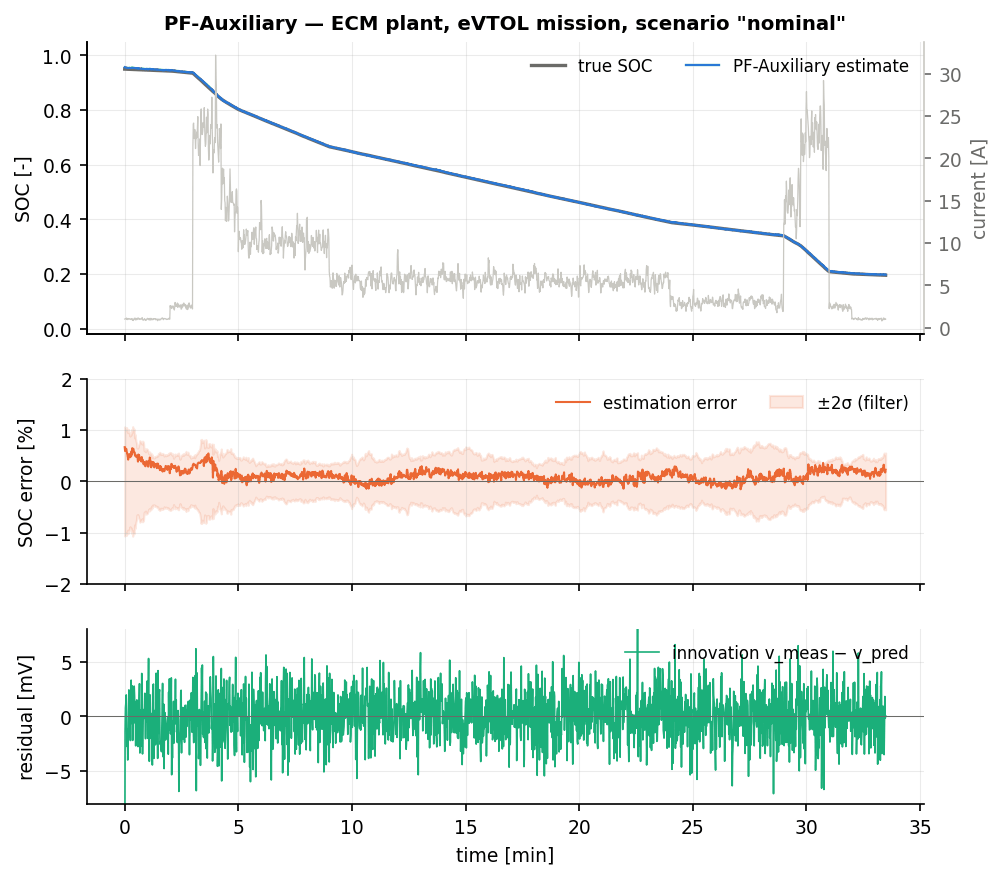
\includegraphics[width=\textwidth]{figures/cell_PFAuxiliary_nominal.png}
\caption{PF-Auxiliary on the nominal eVTOL mission: true and estimated SOC (top), estimation error
with the $\pm2\sigma$ band (middle), voltage residual (bottom).}
\end{figure}
\begin{figure}[H]\centering
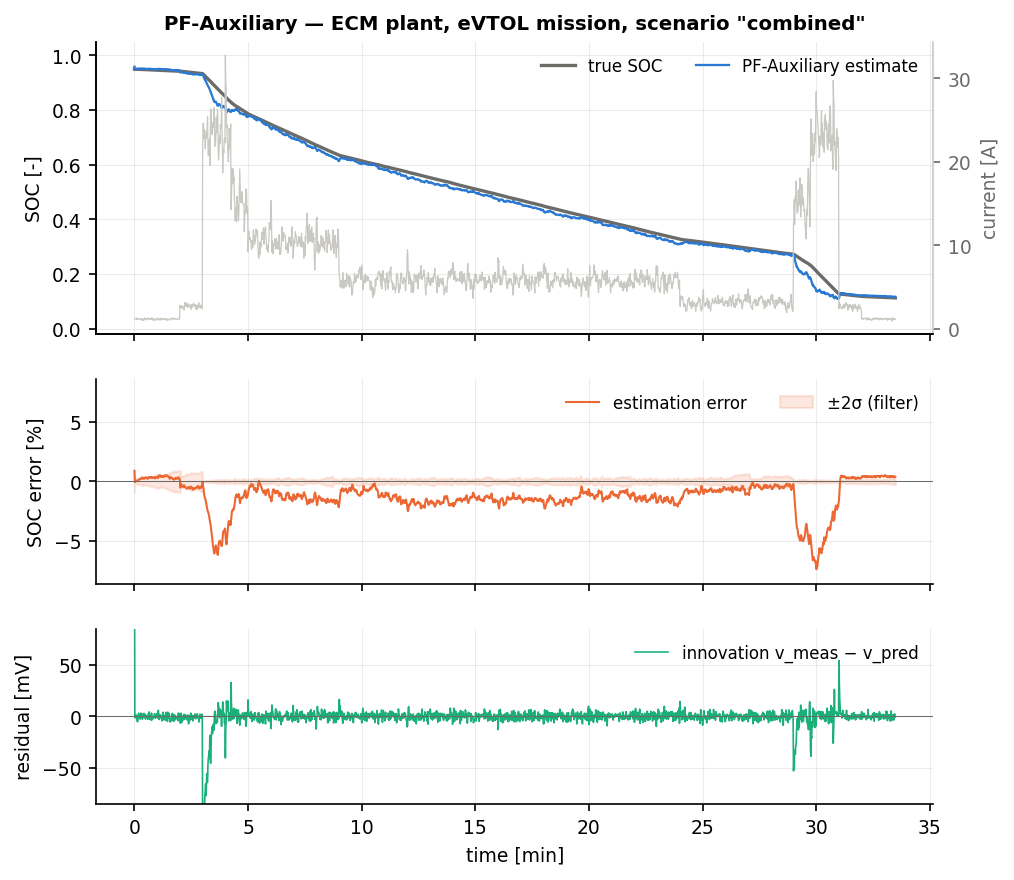
\includegraphics[width=\textwidth]{figures/cell_PFAuxiliary_combined.png}
\caption{PF-Auxiliary on \code{combined} (\SI{25}{\percent} initial error, \SI{0.15}{\ampere}
current bias, \SI{10}{\percent} capacity loss): \SI{2.09}{\percent} steady-state error, the best of
the four full-state particle filters, against \SI{12.44}{\percent} for the EKF.}
\end{figure}
\begin{figure}[H]\centering
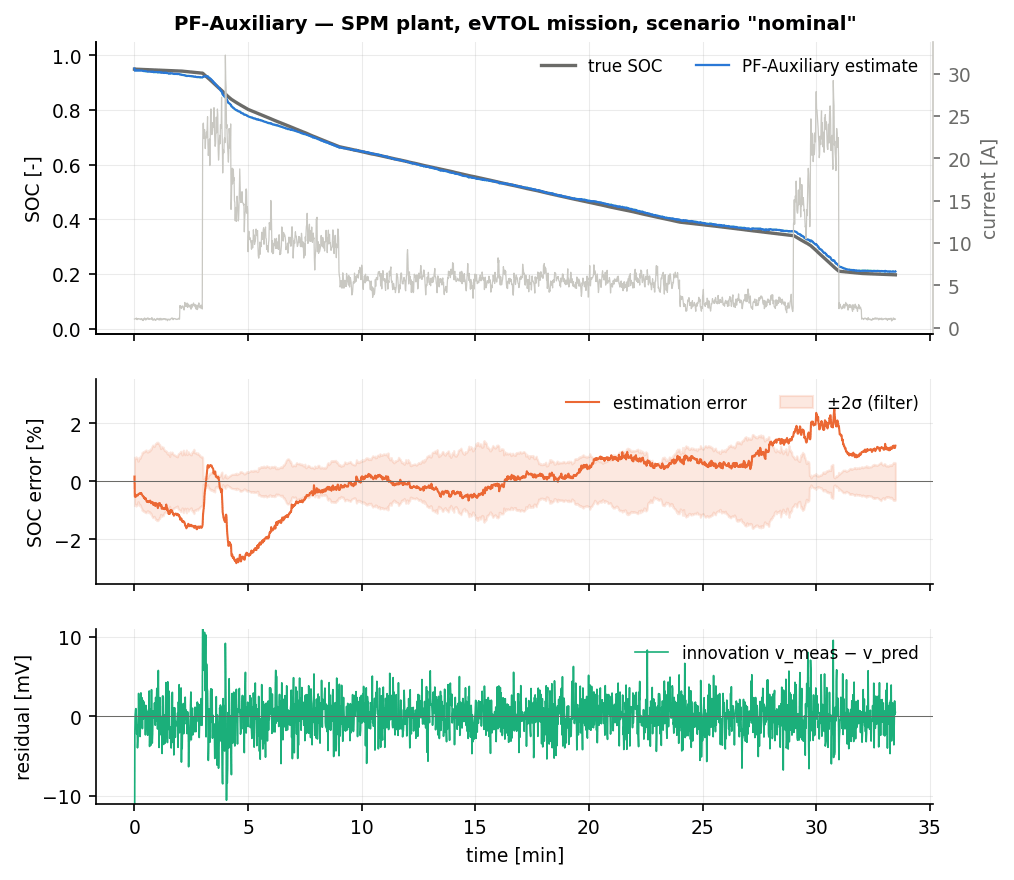
\includegraphics[width=\textwidth]{figures/cellspm_PFAuxiliary_nominal.png}
\caption{PF-Auxiliary on the electrochemical (SPM) plant, nominal mission --- the best steady-state
SOC error of any estimator in this family on that plant (\SI{0.62}{\percent}).}
\end{figure}

\paragraph{ECM plant.}  On \code{nominal} the APF achieves $\mathrm{RMSE} = \SI{0.18}{\percent}$ and
$\mathrm{RMSE}_{\mathrm{ss}} = \SI{0.15}{\percent}$ with a maximum error of \SI{0.88}{\percent} and
immediate convergence --- second of the four full-state particle filters behind the regularised one
(\SI{0.12}{\percent}) and ahead of the bootstrap (\SI{0.16}{\percent}) and fast (\SI{0.18}{\percent})
variants.  All four are far inside the acceptance bound and within Monte-Carlo noise of each other
on this scenario; the interesting separation is elsewhere.

The look-ahead pays off where the likelihood is unusually informative or unusually hostile, and the
pattern is consistent:
\begin{itemize}[leftmargin=2em]
  \item \code{noise\_step} --- \SI{0.34}{\percent}, the best of the four (bootstrap
        \SI{0.51}{\percent}, regularised \SI{0.50}{\percent}, fast \SI{0.68}{\percent}).  When
        $\sigma_v$ jumps to \SI{20}{\milli\volt} the fixed $\mR$ makes all bootstrap weights too
        aggressive; the APF's ratio \eqref{eq:apf-w2} partially cancels the mis-specification
        because the same wrong $\mR$ appears in numerator and denominator.
  \item \code{param\_mismatch} \SI{1.63}{\percent} and \code{aged\_cell} \SI{2.39}{\percent} --- the
        best of the four, although still short of the EKF's \SI{1.36}{\percent} and
        \SI{1.52}{\percent} on a plant whose structure is exact.
  \item \code{combined} \SI{2.09}{\percent}, the best of the four and a factor of six better than
        the EKF's \SI{12.44}{\percent}.
  \item \code{sensor\_dropout} \SI{0.12}{\percent} with a maximum error of only \SI{0.95}{\percent},
        the smallest transient of the whole family: during the \SI{15}{\second} of frozen voltage
        the look-ahead and the realised likelihood agree almost exactly, so the weights stay uniform
        and the filter coasts on the dynamics.
\end{itemize}
The cost of the look-ahead shows in the initial-error recovery, \SI{155}{\second} against
\SI{9}{\second} for \estname{PF-Regularized}: with $K=0$ the jitter floor is set to \num{0.002} of
prior standard deviation instead of \num{0.005}, so the cloud walks more slowly, and the very
selectivity that makes the APF efficient also concentrates the first-stage weights onto the few
parents in the upper tail.  The steady-state error after that recovery, \SI{0.12}{\percent}, is
second best of the four.  Like every particle filter here it loses to the EKF on \code{preisach}
(\SI{1.07}{\percent} against \SI{0.20}{\percent}) under the corrected hysteresis sign convention.

\paragraph{SPM plant.}  This is where the auxiliary stage is most convincing.  On the
electrochemical plant \estname{PF-Auxiliary} gives $\mathrm{RMSE}_{\mathrm{ss}} =
\SI{0.62}{\percent}$ on \code{nominal} --- the best of every estimator in this family --- against
\SI{3.73}{\percent} for the EKF and \SI{3.96}{\percent} for the UKF, a factor of six.  It leads the
family on \code{param\_mismatch} (\SI{1.01}{\percent} against the EKF's \SI{3.13}{\percent}),
\code{current\_bias} (\SI{0.89}{\percent} against \SI{5.69}{\percent}), \code{hot}
(\SI{0.59}{\percent} against \SI{2.16}{\percent}) and \code{sensor\_dropout} (\SI{0.69}{\percent}
against \SI{5.31}{\percent}), and nothing diverges.

Two mechanisms combine.  The first is the one common to all the full-state particle filters: the
roughening jitter keeps the slow RC state free, so the structured \SI{4}{\milli\volt} residual is
taken up by $v_2$ and by the voltage residual rather than by SOC, and the cloud is never forced into
the linearised $(\soc,v_2)$ trade-off that a Kalman gain must make.  The second is specific to the
auxiliary stage and is what puts it ahead of the others: under a persistent model error the
look-ahead likelihood $p(\vy_k\mid\bm\mu^i)$ and the realised likelihood $p(\vy_k\mid\vx_k^j)$ are
biased in the \emph{same} direction, so the ratio \eqref{eq:apf-w2} cancels most of the bias and
the second-stage weights stay near uniform.  The filter therefore keeps a well-populated cloud
exactly when the other variants are spending their effective sample size on a residual none of
their particles can explain.  The price is \SI{443}{\second} to converge on SPM \code{init\_error}
and \SI{986}{\second} on SPM \code{cold}, both scenarios in which the slow diffusion of the SPM has
to be worked out of the RC states before the SOC error can be resolved.

\section{Summary}
The auxiliary particle filter resamples before it propagates, using a one-step preview of the
likelihood to decide which parents deserve the expense of a child.  When the process noise is small
relative to the measurement information --- the permanent condition of a battery SOC estimator ---
the second-stage weights are nearly uniform and the filter approaches the efficiency of independent
sampling from the posterior.  On the ECM plant it then delivers the best results of the four
full-state particle filters on every biased scenario (\code{aged\_cell} \SI{2.39}{\percent},
\code{param\_mismatch} \SI{1.63}{\percent}, \code{combined} \SI{2.09}{\percent}) and the smallest
sensor-dropout transient in the library; on the electrochemical plant it is the most accurate
estimator of the whole family (\SI{0.62}{\percent} against the EKF's \SI{3.73}{\percent}).  It costs
one extra evaluation of $h$ per particle (\SI{104}{\micro\second}/step, the most expensive method in
this family) and it is \emph{not} a universal improvement: with large process noise the ratio
$p(\vy\mid\vx)/p(\vy\mid\bm\mu)$ becomes erratic and the APF can fall behind the bootstrap filter.
Choose it when the model is suspect and the sensor is good; choose the regularised filter when the
initial uncertainty dominates; choose neither if a Kalman filter will do and the model is trusted.
